\documentclass[letterpaper,10pt,conference]{ieeeconf}
\usepackage{times}
\usepackage[numbers]{natbib}
\usepackage{multicol}
\usepackage[bookmarks=true]{hyperref}

\usepackage{lipsum}
\usepackage{comment}
\usepackage{balance}
\usepackage{graphicx}
\usepackage[table]{xcolor}
\usepackage{caption}
%\captionsetup[table]{labelformat=empty}
\usepackage{listings}
% ==================================
% I ADDED THIS FOR CODE PARTS
\usepackage{xcolor}

\definecolor{codegreen}{rgb}{0,0.6,0}
\definecolor{codegray}{rgb}{0.5,0.5,0.5}
\definecolor{codepurple}{rgb}{0.58,0,0.82}
\definecolor{backcolour}{rgb}{0.95,0.95,0.92}

\lstdefinestyle{mystyle}{
    backgroundcolor=\color{backcolour},
    commentstyle=\color{codegreen},
    keywordstyle=\color{magenta},
    numberstyle=\tiny\color{codegray},
    stringstyle=\color{codepurple},
    basicstyle=\ttfamily,
    breaklines=true,
    captionpos=b,
    keepspaces=true,
    numbers=left,
    numbersep=5pt,
    showstringspaces=false,
    tabsize=2
}
\lstset{style=mystyle, language=Python}
% ==================================

% ==================================
% CODE PARTS FROM DANNY PAPER
\usepackage{minted}
\usepackage{xcolor}
\definecolor{bg}{HTML}{f2f2ea}
\usepackage{float} % to force code snippets in place no matter what with H instead of h!
% ==================================



\lstset{
  basicstyle=\ttfamily,
  breaklines=true,
  postbreak=\mbox{\textcolor{red}{$\hookrightarrow$}\space},
}

\usepackage{seqsplit}

\usepackage{amssymb}
\usepackage{amsmath}
\usepackage{booktabs}
 
\usepackage{graphicx} 
\usepackage{subcaption}


\IEEEoverridecommandlockouts
\overrideIEEEmargins

\title{\Large \bf
Learning Event-Aligned Spline Actions for Language-Guided Robot Manipulation
}

\author{Author names removed for blind review.}

% Supplied class title-area hook: no changes to margins or caption typography.
\makeatletter
\newcommand{\teasercaption}[1]{{\def\@captype{figure}\caption{#1}}}
\makeatother
\IEEEaftertitletext{\begin{minipage}{\textwidth}
\centering
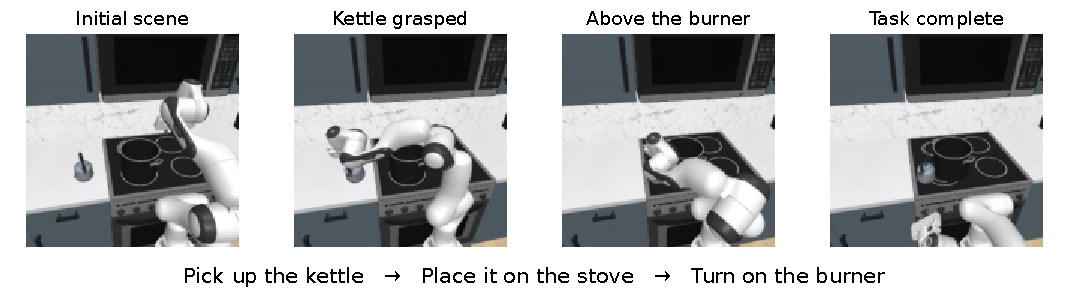
\includegraphics[width=\textwidth]{figures/teaser_v2.pdf}
\teasercaption{A RoboCasa365 policy executes a kettle task through short language instructions. Each instruction conditions several event-aligned spline segments, each with its own predicted duration. The representation exposes two interfaces: which subgoal to execute and how to time its motion. Frames show one successful rollout; text below abbreviates the program, not the active instruction at each displayed frame.\label{fig:teaser}}
\vspace{10pt}
\end{minipage}}

\begin{document}
\maketitle
\thispagestyle{empty}
\pagestyle{empty}

\begin{abstract}
Long-horizon instructions describe a sequence of semantic events, yet vision--language--action (VLA) policies usually emit fixed-rate waypoint arrays that entangle path geometry, execution time, and task progress. We introduce \emph{language-addressable spline action programs}: a VLA action head that represents motion by eight B-spline control points and a learned event duration, and executes an instruction as an ordered sequence of language clauses. This interface leaves the vision--language backbone unchanged while exposing compact, event-aligned units that can be scheduled semantically and resampled in time. In a controlled three-seed study on LIBERO-Long using identical demonstrations and exact replay, clauses improve waypoint success by 34.3 percentage points and spline success by 43.7 points. The additional spline benefit is 9.33 points (hierarchical 95\% CI, 0.67--18.0). Reversing clause order causally changes the first completed subgoal, and semantic phases transfer the effect to RoboCasa365. The learned duration predicts held-out event times (Pearson $r=.819$) and also enables time control: on 3,000 paired CALVIN chains, decode-time retiming improves average chain length by 0.379 while executing 1.42$\times$ faster. Thus, the same action representation strengthens piecewise language execution and provides direct control over a policy's physical clock.
\end{abstract}

\section{Introduction}
\label{sec:introduction}

Vision--language--action policies map natural-language goals and images directly to robot motion \cite{kim2024openvla,black2024pi0,shukor2025smolvla}. Their language input is semantic and hierarchical---``put the soup and tomato in the basket'' implies multiple object-conditioned stages---but their output interface is typically a uniform array of future joint or end-effector waypoints. This mismatch becomes consequential over long horizons. A fixed chunk has neither an explicit semantic boundary nor an independent physical clock, so language must select a behavior, encode its detailed geometry, and implicitly determine how long it should run through the same dense output array.

We ask whether the action interface itself can make a VLA easier to address with language. Our answer is a \emph{language-addressable spline action program} (\method; Fig.~\ref{fig:overview}). Each policy query predicts a compact cubic B-spline trajectory, a gripper curve, and the duration to the next manipulation event. A long instruction is represented as executable clauses; each clause conditions the same policy until a clock advances the program. Normalized spline phase $u\in[0,1]$ represents trajectory shape, while duration $T$ supplies physical time. This separation also makes rate and speed changes decode-time operations on a fixed learned geometry.

The central question is not whether language decomposition helps in general, but whether the action representation changes how much it helps. We therefore conduct a matched $2\!\times\!2$ experiment: stock 50-waypoint SmolVLA versus the spline-duration head, crossed with a whole-task caption versus executable clauses. All four conditions use exactly the same 71 demonstrations and 19,378 physical frames; only the action targets and text view change. Across three training seeds on two LIBERO-Long tasks, clauses improve waypoint success by 34.3 percentage points (pp) and spline success by 43.7~pp. The difference-in-differences is +9.33~pp and is positive for every seed (hierarchical 95\% CI, 0.67--18.0). Static compound-prompt controls regress, showing that the gain comes from executing the language units rather than merely fine-tuning on longer text.

Behavioral interventions and cross-domain tests support the mechanism. Reversing the clause order changes the requested first completed object in 10/50 paired LIBERO states for each head, with no changes in the opposite direction. Official semantic phases raise two-task RoboCasa365 success from 4/100 to 16/100 on one seed and from 3/40 to 9/40 on an independent seed. Finally, the same geometry--time factorization yields a second, complementary capability: retiming a learned spline on CALVIN improves average five-instruction chain length by 0.379 while increasing realized speed by 1.42$\times$, and resampling repairs a LIBERO control-rate failure from 38\% to 68\% and from 34\% to 72\% under two protocols.

\begin{figure*}[t]
    \centering
    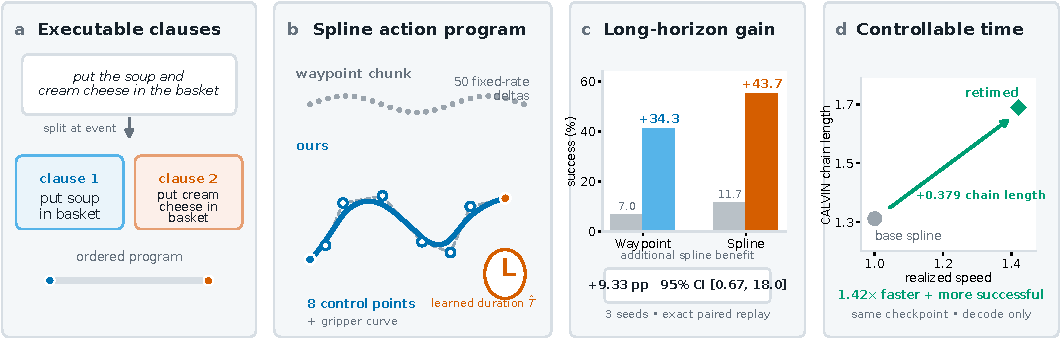
\includegraphics[width=\textwidth]{figures/overview.pdf}
    \caption{\textbf{Language-addressable spline action programs.} A long-horizon instruction is scheduled as executable clauses. For each clause, the VLA predicts eight control points for a continuous path, a gripper curve, and event duration $T$, rather than a dense fixed-rate waypoint array. The matched experiment isolates an additional +9.33~pp clause benefit for the spline head; the same shape--time factorization supports successful decode-time retiming on CALVIN.}
    \label{fig:overview}
\end{figure*}

Our contributions are:
\begin{itemize}
    \item an event-aligned spline VLA head that jointly predicts compact path geometry, gripper state, and physical duration without modifying the vision--language backbone;
    \item a controlled, three-seed executable-language study showing that clauses improve both action heads but improve the spline head significantly more, together with order interventions and RoboCasa365 replication; and
    \item a unified time-control study showing that the same learned head supports event scheduling, language-conditioned pace, temporal rescaling, and control-rate adaptation at decode time.
\end{itemize}

\section{Related Work}
\label{sec:related_works}

\textbf{Action representations.}
Action chunking stabilizes imitation policies by predicting several future actions per query \cite{zhao2023act,chi2023diffusion}. Modern VLAs instantiate this idea with autoregressive tokens or flow-matching experts \cite{pertsch2025fast,black2024pi0,shukor2025smolvla}. Closest to our representation, BEAST compresses continuous action sequences into B-spline tokens \cite{zhou2025beast}; B-spline Policy predicts continuous curves that can be resampled and manually time-scaled \cite{han2026bsp}; and Spline Policy studies spline outputs across policy families, including editing, uncertainty, and controller compatibility \cite{tian2026spline}. We do not claim the first spline head, smooth decoding, or arbitrary-rate resampling. We instead learn the physical duration to the next manipulation event and test a new interaction: whether this event-aligned representation amplifies the benefit of executing language piece by piece.

\textbf{Long-horizon language control.}
Large VLAs use heterogeneous co-training and semantic prediction to execute extended tasks \cite{black2025pi05}, while Long-VLA introduces phase-aware inputs \cite{fan2025longvla}. VLAs-as-Tools delegates planning and progress monitoring to a high-level VLM that invokes specialized policies \cite{lei2026tools}. In contrast, \method{} keeps one end-to-end VLA and makes its action units directly addressable by an ordered clause list. Counterfactual studies show that policies can override language with visual shortcuts \cite{glossop2025cast,fang2026counterfactual}; accordingly, we complement success with paired order and wrong-instruction interventions. This follows the broader lesson from inference-time policy steering that alignment requires measuring whether the requested behavior changes, not merely whether a rollout remains valid \cite{wang2025itps}.

\textbf{When to replan and how fast to act.}
PACE selects a replanning horizon at inference time from low-speed transitions in a predicted action chunk \cite{nie2026pace}. Our event labels supervise time-to-event directly, coupling a language clause to a physical clock. Decoding the same geometry on a warped or denser time grid connects that clock to speed and control-rate adaptation. This timing capability is not our sole novelty; it closes the loop between semantic program progress and continuous robot execution.

\section{Language-Addressable Spline Action Programs}
\label{sec:method}

Let a VLA policy $\pi_\theta$ receive image observations $o_t$, robot state $s_t$, and language $\ell_t$. A conventional chunking policy predicts a fixed sequence $[a_t,\ldots,a_{t+H-1}]$. We replace only this output target and its decoder; the visual encoder, language model, and flow-matching action expert remain unchanged.

\subsection{Shape--Time Factorization}

For an action segment of duration $T$, define the cumulative commanded end-effector path $p_0=0$ and $p_k=\sum_{j<k}a^{\mathrm{pose}}_j$. We represent this path by a clamped, uniform cubic B-spline
\begin{equation}
    p(u)=\sum_{i=0}^{n-1}B_{i,3}(u)c_i, \qquad u=t/T\in[0,1],
    \label{eq:spline}
\end{equation}
with $n=8$ control points. Endpoints are pinned, $c_0=0$ and $c_{n-1}=p_T$; the interior controls minimize $\sum_{k=0}^{T}\|p(k/T)-p_k\|_2^2$. We precompute the resulting least-squares operators for every allowed $T$, reducing target construction and decoding to batched matrix products. A separate spline fits the raw binary gripper command and is thresholded by sign at decode.

One policy output token represents one pose and gripper control point. An eighth supervised channel contains $\log T$, replicated over the eight tokens and averaged at decode. Thus the action expert emits eight structured tokens instead of 50 waypoint tokens. Targets are standardized per token inside the policy; the external action processor is the identity so that decoded deltas retain their physical meaning. We train with SmolVLA's original conditional flow-matching objective \cite{lipman2023flow,shukor2025smolvla}, applied to these transformed targets.

\subsection{Event-Aligned Targets}

Fixed windows often bisect grasps or contacts. We instead terminate a training target at the first event after a minimum of eight steps: (i) a gripper-sign transition, (ii) two consecutive pose speeds below $0.15$ times the within-window median, or (iii) episode end. If none occurs, the segment is capped at 24 steps (16 for 10-Hz CALVIN). The selected endpoint gives both the path-fitting interval and duration label. This construction makes $T$ a supervised time-to-event rather than an arbitrary chunk size.

At inference, the model predicts $\hat T=\exp(\frac{1}{n}\sum_i\widehat{\log T}_i)$, clamped to the training range. Sampling Eq.~\eqref{eq:spline} at $h$ phases $u_j$ gives positional commands $p(u_j)$; differences $p(u_j)-p(u_{j-1})$ recover executable delta actions. Replanning at $\hat T$ therefore aligns policy queries to predicted manipulation events.

\subsection{Executable Language Clauses}

A long instruction is represented as an ordered program $\mathcal{L}=(\ell^1,\ldots,\ell^M)$. The active clause replaces the whole-task caption in the ordinary VLA language input; no planner, tool library, or architecture change is introduced. For the main two-subgoal study, demonstrations are split at the first gripper release following at least 48 consecutive closed commands. The release remains under clause 1 and the next observation/action pair begins clause 2. All images, states, actions, episode indices, and optimization schedules are otherwise identical to the whole-caption dataset.

During execution a scheduler advances the clause pointer and clears actions generated under the preceding clause. The primary head comparison uses the same outcome-independent clock for waypoint and spline policies: the task-specific median causal switch frame from the training demonstrations (139 and 107 steps). This isolates the action-representation interaction. A second deployment condition advances on the policy's predicted close-to-open gripper event; a separate privileged predicate scheduler is used only for the diagnostic order intervention. The duration channel independently controls when the policy replans within each clause.

\subsection{One Curve, Multiple Physical Clocks}

Because $p$ is parameterized by normalized phase, timing changes need not alter its learned geometry. A monotone time map $\phi:[0,1]\!\rightarrow\![0,1]$ produces $p(\phi(u))$: uniform compression changes overall pace, while interval-selective warping protects slow contact regions. Sampling $p$ at $h=\rho\hat T$ rather than $\hat T$ changes control rate by ratio $\rho$ while preserving endpoints and nominal velocity. If any decoded delta exceeds an actuator bound, feasibility stretch increases $h$ until the bound is met. These operations use one checkpoint and require no additional policy queries or neural inference.

\section{Experiments}
\label{sec:experiments}

We evaluate four questions: (Q1) Does the structured head preserve ordinary VLA competence? (Q2) Do executable clauses improve long-horizon execution, and does the spline head benefit more? (Q3) Does changing a clause change the corresponding behavior? (Q4) Does separating shape and time enable useful deployment control?

\subsection{Setup}

\textbf{Policies.} All policies use the 450M-parameter SmolVLA backbone \cite{shukor2025smolvla}. We compare \textbf{A}, stock 50-waypoint SmolVLA; \textbf{B}, eight-control-point cubic splines over a fixed 20-step window; and \textbf{C}, our event-aligned spline with learned duration. A and C are the matched heads in language experiments. Unless noted, policies execute 10 actions before replanning. Training seeds vary both optimization and action-expert initialization.

\textbf{Training.} The broad LIBERO comparison trains every head for 100,000 updates with batch size 32 on the identical 40-task dataset, using seeds 1000--1002 and the same pretrained SmolVLM initialization. The clause factorial starts from the corresponding 100k A or C checkpoint and applies 7,500 matched updates (batch 32) to one frozen 71-episode manifest. RoboCasa label comparisons likewise hold initialization, physical episodes, update count, and optimizer schedule fixed within each seed. All timing and rate variants are configuration-only decodes of an already trained checkpoint unless explicitly labeled as a language or retrained baseline.

\textbf{Domains and metrics.} LIBERO \cite{liu2023libero} supplies four ten-task suites and the two multi-object LIBERO-Long tasks used for the clause factorial. We report task success. CALVIN \cite{mees2022calvin} uses the official five-instruction chain protocol; its metric is the mean number of consecutive tasks completed. RoboCasa365 \cite{nasiriany2026robocasa365} tests mobile manipulation in diverse kitchens. Paired comparisons use identical initial simulator states and policy seeds. Exact-replay gates hash initial observations, simulator states, prompts, and complete action traces; all 30 clause-study gates passed across 6,000 control and treatment rollouts.

\subsection{Q1: Broad Competence Is Preserved}

Table~\ref{tab:libero} reports three training seeds and 1,200 rollouts per arm across four suites (300 per suite). A Barnard test with Bonferroni correction finds no significant arm difference after protocol crossing. C is within 1.4 points of waypoint SmolVLA overall and has the lowest across-seed variation, so the new interface does not purchase its downstream capabilities by sacrificing broad success.

\begin{table}[t]
\centering
\caption{LIBERO success (\%, three training seeds). ``Avg.'' averages the four suites; $\pm$ is its seed standard deviation.}
\label{tab:libero}
\setlength{\tabcolsep}{3.5pt}
\begin{tabular}{lrrrrrr}
\toprule
Head & Obj. & Spatial & Goal & Long & Avg. & SD \\
\midrule
A Waypoint & 94.7 & 84.3 & 86.0 & 63.3 & \textbf{82.1} & 1.8 \\
B Fixed spline & \textbf{96.3} & 77.7 & 84.0 & \textbf{65.3} & 80.8 & 2.5 \\
C Spline+duration & 92.3 & 77.3 & \textbf{89.3} & 63.7 & 80.7 & \textbf{1.3} \\
\bottomrule
\end{tabular}
\end{table}

\begin{figure*}[t]
    \centering
    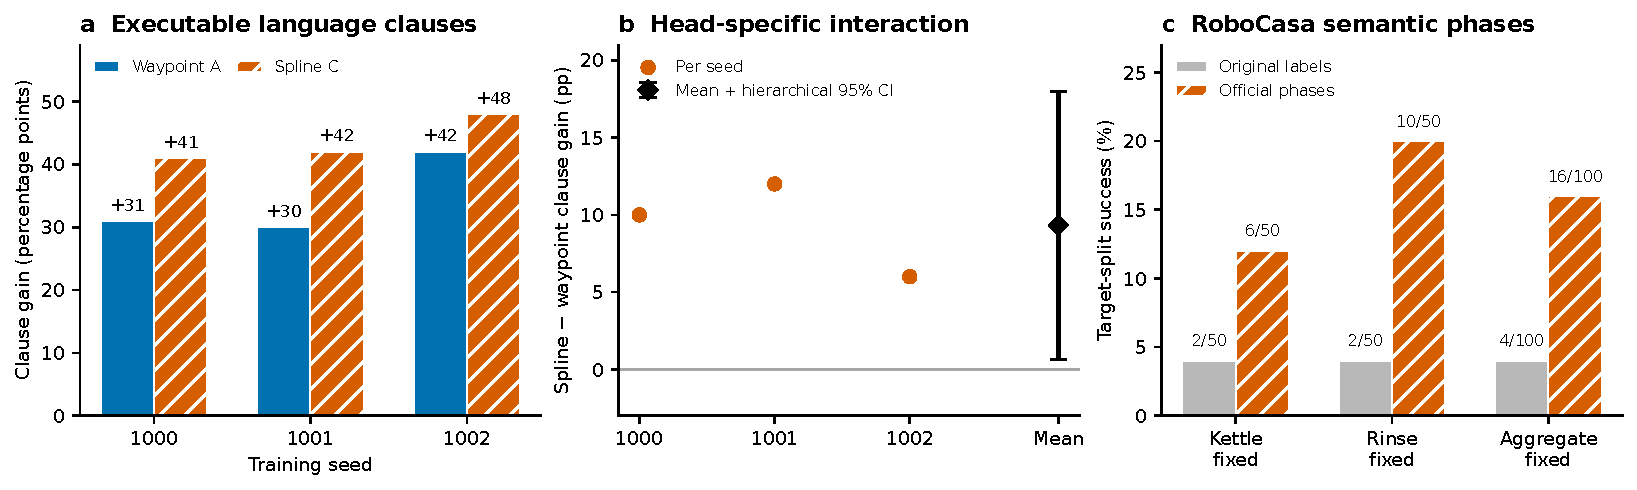
\includegraphics[width=\textwidth]{figures/headline_results.pdf}
    \caption{\textbf{Executable-language results.} (a) Clauses improve both heads on two LIBERO-Long tasks and all training seeds. (b) Their gain is consistently larger for the event-aligned spline head; the hierarchical interval excludes zero. (c) Official semantic phases improve the first-seed RoboCasa365 target split. The independent-seed replication appears in Table~\ref{tab:robocasa}.}
    \label{fig:headline}
\end{figure*}

\subsection{Q2: Executable Clauses Improve Long-Horizon Tasks}

An initial Molmo-2 segment-label pilot moved t0 from 24/50 to 38/50 while leaving the ten-task suite approximately flat; it motivated a cleaner exact-clause intervention.

The controlled study contains 33 demonstrations of LIBERO-Long t0 (soup and tomato into a basket) and 38 of t4 (two mugs onto different plates): 71 episodes and 19,378 frames total. Whole-caption and clause datasets are byte-identical in every non-language column. Within each head, the two language treatments receive the same head-matched 100k-step warm start, episodes, batch size, and 7,500-step budget.

Figure~\ref{fig:headline}a shows the aggregate result over 50 states per task. Pooled across seeds, A rises from 7.0\% to 41.3\% and C from 11.7\% to 55.3\%. Clauses improve A by 31, 30, and 42~pp across seeds and C by 41, 42, and 48~pp. The mean gains are 34.33 and 43.67~pp, respectively. The difference-in-differences,
\begin{equation}
  \Delta_{\mathrm{head}}=(C_{\mathrm{clause}}-C_{\mathrm{whole}})
       -(A_{\mathrm{clause}}-A_{\mathrm{whole}}),
\end{equation}
is +10, +12, and +6~pp (mean +9.33~pp). A hierarchical bootstrap over training seeds and paired states gives a 95\% CI of 0.67--18.0~pp; the seed-level $t$ interval is 1.74--16.92~pp. This establishes an action-representation interaction, not merely an advantage from adding labels.

Two controls isolate execution from relabeling. First, clause-trained policies evaluated once with a static compound prompt regress by 9.33~pp (A) and 24.0~pp (C) relative to their original-label counterparts. Second, advancing C on its predicted close-to-open gripper event retains a 40.33~pp mean clause gain, comparable to the matched fixed-clock gain. Clause-conditioned C also succeeds faster descriptively on seed 1000 (median steps t0, 321$\rightarrow$270; t4, 292$\rightarrow$236).

\subsection{Q3: Language Changes the Requested Behavior}

We reverse the two clauses and score which official goal predicate is reached first. A privileged predicate transition advances the program in this diagnostic only. On t4, both A and C change the first completed object in the requested direction on 10/50 paired states, with zero opposite-direction changes (two-sided sign test $p=.00195$). Of 12 states with a unique first goal under both orders, 10 flip as requested. Final conjunction success falls from 49/100 to 16/100 for A and from 55/100 to 21/100 for C: language can redirect the first subgoal, but canonical-order bias still impairs retention and completion. This distinction prevents first-subgoal steering from being mistaken for solved compositional generalization.

\subsection{RoboCasa365 Semantic Phases}

RoboCasa's longer manipulation sequences test whether short language units remain useful beyond LIBERO. We relabel identical physical demonstrations using the benchmark's official semantic phases: pick, place, and actuate for KettleBoiling; faucet and basin-washing phases for RinseSinkBasin. Policies use an outcome-independent fixed phase clock. Table~\ref{tab:robocasa} shows that the two-task aggregate improves on both training seeds. Rinse replicates strongly; Kettle is heterogeneous.

\begin{table}[t]
\centering
\caption{RoboCasa365 target-split full-task success. Each cell is original labels $\rightarrow$ official phase labels.}
\label{tab:robocasa}
\setlength{\tabcolsep}{4pt}
\begin{tabular}{crrr}
\toprule
Seed & Kettle & Rinse & Aggregate \\
\midrule
1000 & 2/50$\rightarrow$6/50 & 2/50$\rightarrow$\textbf{10/50} & 4/100$\rightarrow$\textbf{16/100} \\
1001 & 2/20$\rightarrow$1/20 & 1/20$\rightarrow$\textbf{8/20} & 3/40$\rightarrow$\textbf{9/40} \\
\bottomrule
\end{tabular}
\end{table}

The aggregate gains are +12 and +15~pp (4$\times$ and 3$\times$ the original counts), for an unweighted mean gain of 13.5~pp. On seed 1000, phase labels increase Kettle grasps from 24/50 to 39/50 ($p=.00346$) and Rinse rollouts reaching water-on/one washed region from 7/50 to 22/50 ($p=.00175$). The latter mechanism replicates 3/20$\rightarrow$12/20 on seed 1001 ($p=.00791$). Figure~\ref{fig:kettle} localizes a matched Kettle outcome: both policies grasp and place from the same initial state, but only phase supervision preserves progress through burner actuation.

\begin{figure*}[t]
    \centering
    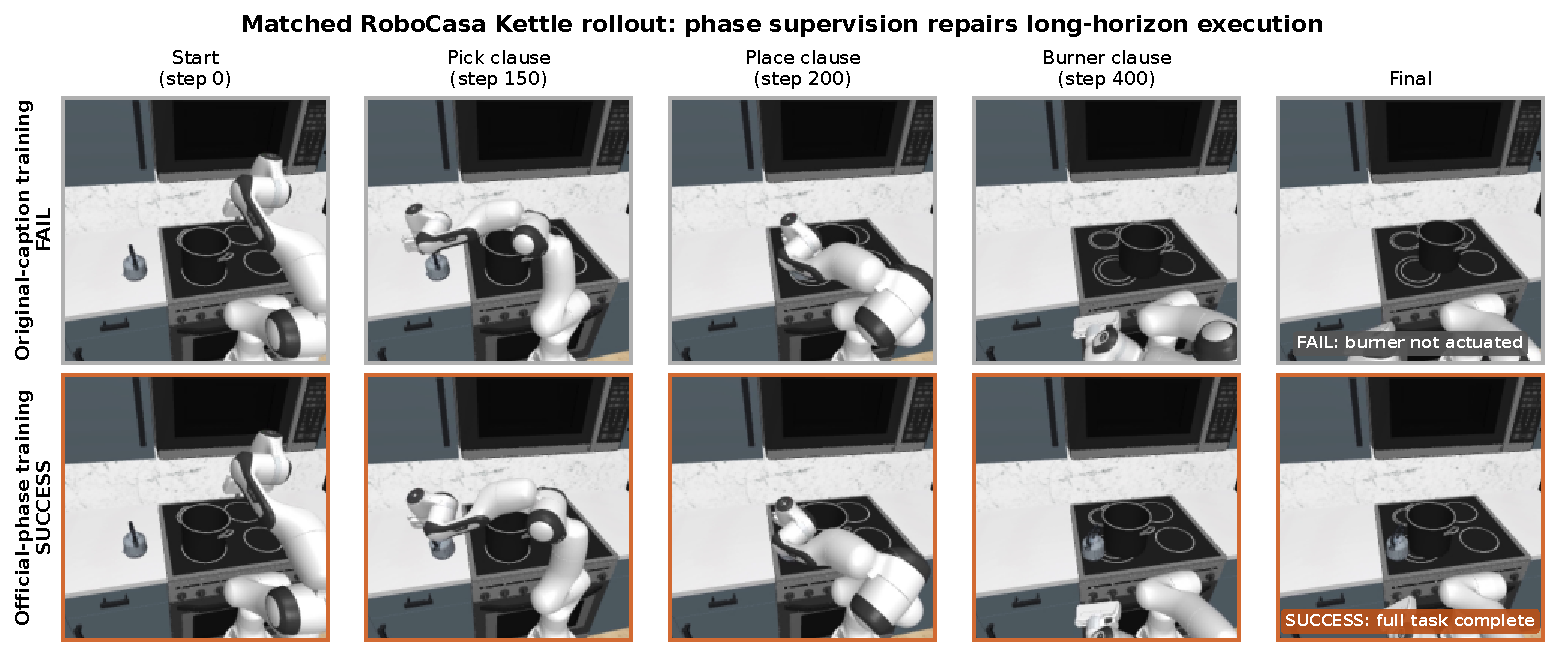
\includegraphics[width=\textwidth]{figures/kettle_phase_storyboard.pdf}
    \caption{\textbf{Matched RoboCasa365 Kettle rollout.} The original-caption and official-phase policies share the exact initial observation. Both reach grasp and stove contact at similar times; only the phase-trained policy completes burner actuation (516 steps versus failure at the 1,500-step limit).}
    \label{fig:kettle}
\end{figure*}

Wrong-instruction controls confirm prompt sensitivity in atomic tasks: changing drawer left$\leftrightarrow$right reduces A/C success from 7/50 and 6/50 to zero; rack in$\leftrightarrow$out reduces 18/50 and 15/50 to zero. Since the reward still scores the original goal, these controls establish suppression of an incompatible behavior, not alternate-goal completion.

\subsection{Q4: The Learned Physical Clock Is Controllable}

The duration head predicts held-out event times with 1.61-step MAE and Pearson $r=.819$; event-versus-cap balanced accuracy is .892. Figure~\ref{fig:control} reports absolute outcomes before paired differences so that every gain has an explicit comparator. On CALVIN, waypoint A averages 1.56 completed tasks, unretimed C averages 1.31, and uniformly retimed C averages 1.69. Every C seed improves under the same decode-only intervention. The paired gain over C-base is 0.379 (95\% CI, 0.318--0.441) at 1.42$\times$ realized speed; retimed C also exceeds waypoint A by 0.127 (CI, 0.063--0.191) while matching first-task success (69.9\% versus 69.4\%, McNemar $p=.56$). Both contrasts pool three seeds and 1,000 identical official chains per seed.

\begin{figure*}[t]
    \centering
    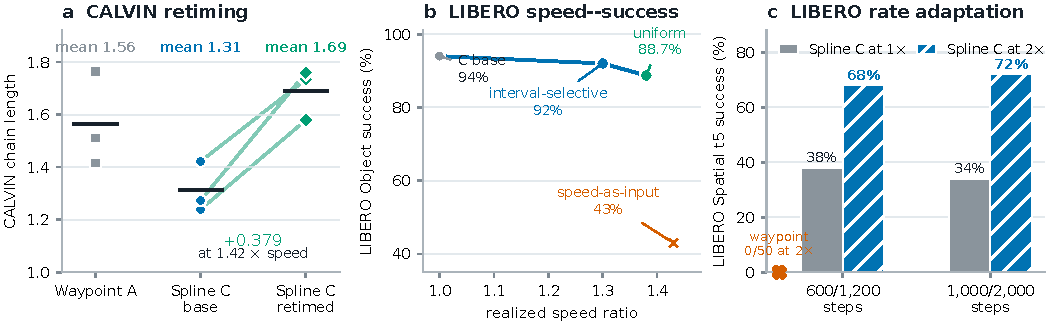
\includegraphics[width=\textwidth]{figures/control_results.pdf}
    \caption{\textbf{Timing and control-rate results.} (a) Absolute CALVIN chain length for three training seeds; horizontal ticks are means and lines connect each C-base seed to its retimed counterpart. Uniform retiming recovers the unretimed spline deficit and exceeds waypoint A while executing faster. (b) On LIBERO Object, the same C checkpoint traces a speed--success frontier; the separately retrained speed-as-input baseline collapses near the same speed. (c) Sampling the same spline at twice the control rate repairs LIBERO Spatial t5 under two independently budgeted horizon protocols; direct waypoint replay fails on the measured $2\times$ condition.}
    \label{fig:control}
\end{figure*}

The LIBERO panels separate two uses of time. Retiming changes how quickly normalized phase is traversed: interval-selective compression retains 92\% success at 1.30$\times$, versus 94\% for C-base, while uniform compression reaches 1.38$\times$ at 88.7\%. A budget-matched speed-as-input policy requires retraining yet reaches only 43\% at 1.43$\times$. Rate adaptation instead samples the same curve more densely. At $2\times$ control rate, C improves from 38\% to 68\% and from 34\% to 72\% under two paired horizon protocols; direct waypoint replay is 0/50. The gain is task-selective---the full Spatial suite remains approximately flat---and is therefore a remedy for tracking-limited cells, not a universal success boost.

\begin{table*}[t]
\centering
\caption{Additional uses of the learned spline interface. Each row states what changes relative to the named baseline; $\dagger$ marks a supporting single-seed mechanism cell rather than a headline aggregate.}
\label{tab:control}
\small
\setlength{\tabcolsep}{4pt}
\renewcommand{\arraystretch}{1.08}
\begin{tabularx}{\textwidth}{@{}l X X l@{}}
\toprule
Use & Intervention and comparator & Audited outcome & Evaluation \\
\midrule
Language pace & CALVIN prompt: plain $\leftrightarrow$ ``quickly'' / ``slowly'' & Realized pace $+16\%/-16\%$; plain \mbox{$1.382\rightarrow1.553$} with ``quickly'' ($\Delta=.172$, $p=.018$; Bonferroni $p=.035$) & 600 paired chains/condition \\
Event replanning & Fixed cadence $\rightarrow$ replan at $\hat T-4$ & Matched success with $2.7\times$ fewer policy calls on LIBERO and $2.1\times$ fewer on CALVIN & fixed checkpoints; CALVIN $3\times1{,}000$ \\
Feasibility stretch$\dagger$ & Clip coarse-rate deltas $\rightarrow$ lengthen the execution window until feasible & $+19$ success points at half control rate & paired LIBERO cell \\
Shape capacity$\dagger$ & Long t7: eight $\rightarrow$ twelve control points & 42\%$\rightarrow$78\% success & paired LIBERO cell \\
Execution cadence$\dagger$ & Long t8: same n16/h48 checkpoint, short $\rightarrow$ long execution & 30\%$\rightarrow$52\% success & paired LIBERO cell \\
Failure signal & Threshold a stalled $\hat T$ countdown & 86\% precision / 52\% recall & fixed LIBERO checkpoint \\
Contact ease-out & Linear phase $\rightarrow$ endpoint-preserving cosine warp & Terminal velocity $0.14\times$ with identical endpoint & offline kinematics \\
Compute & Waypoint A $\rightarrow$ spline C policy call & 209.1$\rightarrow$221.7~ms (+6\%); precomputed spline decode $<1$~ms & A40 latency \\
\bottomrule
\end{tabularx}
\end{table*}

Retiming is data-dependent rather than universally beneficial. An imitation policy inherits the demonstrator's time map; compression can harvest dead time, but it can also induce actuator clipping or rush precision-critical contact. Scripted LIBERO contains little removable hesitation, so interval-selective warping loses the least. CALVIN demonstrations contain distributed low-speed dithering, so uniform retiming removes more harmful hesitation and is best. RoboCasa operates near its action bound (38\% of frames exceed 60\% of the bound), so aggressive compression is clipped or re-expanded and becomes success-neutral. Nevertheless, successful Kettle rollouts shorten descriptively from 230 to 97 steps. These measured regimes explain why one decode rule should not be expected to dominate every dataset.

The interface remains efficient because the VLM dominates latency. An A40 policy call increases only 6\% from A to C (Table~\ref{tab:control}); at $2\times$ rate, curve resampling yields twice as many environment steps without an additional neural query. With fixed flow-matching noise, decoding the same tokens at $1\times$ and $2\times$ has approximately zero endpoint/path deviation from the fine reference, while commanded jerk falls from .040 to .0055. Event-scheduled replanning then uses the learned clock to reduce policy calls, rather than merely increasing low-cost interpolation steps.

\subsection{Real-Robot Evaluation}
\label{sec:hardware}

\textit{Protocol frozen; quantitative trials are being collected.} The platform contains two 7-DoF xArm7 manipulators on 1-DoF linear rails, with one arm providing an external camera view and the other executing gripper actions. Demonstrations are collected with a handheld one-arm teleoperation device. Existing 3D-printed fixtures support two focused programs: (i) open drawer $\rightarrow$ insert object $\rightarrow$ close or leave open, enabling a matched late-clause intervention with an identical prefix; and (ii) a physically valid non-cuboid stacking order. The rail remains fixed unless reach requires it.

We will derive whole-caption and clause-labeled datasets from the same physical trajectories and compare A/C$\times$whole/clause whenever all four policies pass seen-program competence. Evaluation uses 20 frozen initial configurations per condition, interleaved treatment order, and reports requested first subgoal, final success, and prefix-versus-late trajectory divergence. A filmstrip and result table will replace this paragraph after the frozen evaluation; no hardware result is assumed in the claims above.

\section{Discussion and Conclusion}
\label{sec:discussion}

The results support a specific claim: piecewise language is useful for both conventional and structured action heads, and an event-aligned spline head benefits more. We attribute this interaction to a better-matched interface. A clause specifies one manipulation phase; eight control points express its geometry; a gripper curve exposes its terminal interaction; and duration supplies its physical clock. The representation does not solve high-level planning by itself, but it reduces the burden placed on a single fixed-rate action array.

The language and timing results also explain one another. Words affect behavior only when demonstrations make them informative. Executable clauses vary within a long task and produce large gains; speed adverbs label physically different continuations and yield bidirectional pace control. By contrast, changing an object word without counterfactually varying the demonstrated target does not overcome a positional shortcut. Similarly, decode-time acceleration helps when demonstrations contain removable dead time (CALVIN), is neutral near actuator limits (RoboCasa), and trades accuracy for speed when scripted trajectories contain little slack (LIBERO). These conditions make the control surface predictable rather than a universal speedup claim.

Our study is presently limited to a 450M-parameter VLA, two claim-bearing LIBERO-Long tasks, and two RoboCasa programs. The order probe establishes causal first-subgoal steering but not robust reversed-order completion. These limitations identify the most direct next test: train on several subgoal combinations and hold out one composition, then evaluate a matched later-clause intervention. The real-robot protocol in Sec.~\ref{sec:hardware} instantiates the same test with drawer and stacking programs. Scaling \method{} to pretrained $\pi_{0.5}$-class backbones is complementary rather than necessary to identify the head-level effect.

In summary, language-addressable spline action programs connect three structures that fixed waypoint chunks leave entangled: semantic subgoals, continuous trajectory shape, and physical time. They preserve broad VLA competence, amplify executable-clause gains, causally steer subgoal order, and expose practical replanning, pace, and control-rate mechanisms from one checkpoint. This combination turns a compact spline from an output compression device into an interface between language and closed-loop robot execution.


\bibliographystyle{ieeetr}
\bibliography{refs}
\end{document}
